\documentclass[hyperref,UTF8,12pt,a4paper]{ctexart}
\usepackage{amsmath}
\usepackage{amsfonts}

\usepackage{geometry}
\usepackage{tikz}
\geometry{left=1in,right=1in,top=1in,bottom=1in}

%% make section title left aligned
% \ctexset{section/format=\Large\bfseries}

%% pseudo-code
\usepackage{algorithm}
\usepackage{algpseudocode}

%% minted
\usepackage{minted}

%% plots
\usepackage{pgfplots}
\pgfplotsset{compat = newest}

\hypersetup{
	colorlinks=true,
	linkcolor=black
}
\ctexset{abstractname=\zihao{2}摘\quad{}要}

\usepackage{titling}
\pretitle{\begin{center}\fontsize{30pt}{30pt}\selectfont}
\posttitle{\end{center}}

\usepackage{appendix}

\usepackage{ulem}

%% header
% \usepackage{fancyhdr}
% \pagestyle{fancy}
% \fancyhf{}
% \fancyhfoffset[L]{0cm} % left extra length
% \fancyhfoffset[R]{0cm} % right extra length
% \chead{鲍鱼年龄预测分析}
% \rhead{\thepage}
% \rfoot{}

\title{鲍鱼年龄预测分析}
\author{罗江楠}
\date{\today}

\begin{document}

% title page
\maketitle
\newpage

% 摘要

\begin{abstract}
  \vspace{\baselineskip}
  关注永雏塔菲喵,关注永雏塔菲谢谢喵。关注永雏塔菲喵,关注永雏塔菲谢谢喵。关注永雏塔菲喵,关注永雏塔菲谢谢喵。关注永雏塔菲喵,关注永雏塔菲谢谢喵。关注永雏塔菲喵,关注永雏塔菲谢谢喵。关注永雏塔菲喵,关注永雏塔菲谢谢喵。关注永雏塔菲喵,关注永雏塔菲谢谢喵。关注永雏塔菲喵,关注永雏塔菲谢谢喵。关注永雏塔菲喵,关注永雏塔菲谢谢喵。关注永雏塔菲喵,关注永雏塔菲谢谢喵。关注永雏塔菲喵,关注永雏塔菲谢谢喵。关注永雏塔菲喵,关注永雏塔菲谢谢喵。关注永雏塔菲喵,关注永雏塔菲谢谢喵。关注永雏塔菲喵,关注永雏塔菲谢谢喵。

  关注永雏塔菲喵,关注永雏塔菲谢谢喵。关注永雏塔菲喵,关注永雏塔菲谢谢喵。关注永雏塔菲喵,关注永雏塔菲谢谢喵。关注永雏塔菲喵,关注永雏塔菲谢谢喵。关注永雏塔菲喵,关注永雏塔菲谢谢喵。关注永雏塔菲喵,关注永雏塔菲谢谢喵。关注永雏塔菲喵,关注永雏塔菲谢谢喵。关注永雏塔菲喵,关注永雏塔菲谢谢喵。关注永雏塔菲喵,关注永雏塔菲谢谢喵。关注永雏塔菲喵,关注永雏塔菲谢谢喵。关注永雏塔菲喵,关注永雏塔菲谢谢喵。关注永雏塔菲喵,关注永雏塔菲谢谢喵。关注永雏塔菲喵,关注永雏塔菲谢谢喵。关注永雏塔菲喵,关注永雏塔菲谢谢喵。关注永雏塔菲喵,关注永雏塔菲谢谢喵。关注永雏塔菲喵,关注永雏塔菲谢谢喵。关注永雏塔菲喵,关注永雏塔菲谢谢喵。关注永雏塔菲喵,关注永雏塔菲谢谢喵。关注永雏塔菲喵,关注永雏塔菲谢谢喵。关注永雏塔菲喵,关注永雏塔菲谢谢喵。

  \textbf{关键词:}关注永雏塔菲喵,关注永雏塔菲谢谢喵
\end{abstract}


% toc
\tableofcontents
\newpage

% 正文
\section{数据处理}

\subsection{数据集信息}

鲍鱼年龄的测量实际上十分复杂,需要将壳切开并染色,接着在显微镜下测量环的数量才能确定。这无疑是一项繁琐而又费时的工作。如果我们可以通过测量一些可以简单测量出来的数据,并通过一个公式能够粗略估计出鲍鱼年龄的话,无疑是一个很好的方法。

加洲大学海湾分校有一组统计的鲍鱼数据集,其中包括了以下的一些信息

\begin{center}
  \begin{tabular}{c c c c}
    \hline
    \hline
    \textbf{字段名} & \textbf{类型} & \textbf{测量单位} & \textbf{备注} \\
    \hline
    性别(Sex) & nominal & / & M, F, and I (infant) \\
    长度(Length) & 连续 & mm & \\
    直径(Diameter) & 连续 & mm & \\
    高度(Height) & 连续 & mm & \\
    整体重量(Whole weight) & 连续 & g & \\
    去壳重量(Shucked weight) & 连续 & g & \\
    内脏重量(Viscera weight) & 连续 & g & \\
    壳重量(Shell weight) & 连续 & g & \\
    环数(Rings) & 整数 & / & \\
    \hline
    \hline
  \end{tabular}
\end{center}

其中环数是一个整数,我们可以通过环数加上 $1.5$ 来直接估计鲍鱼的年龄。

本文来探讨,如何使用这个数据集来简单推导出一个用于估算鲍鱼年龄的公式。

\section{回归分析}

在进行统计分析之前,我们将所有的环数数据都加上了 $1.5$,并将其变为了新的 age 字段。

\subsection{建立回归模型}

在建立回归模型之前,我们先来计算一下数据集中各变量之间的相关性。

\begin{minted}{text}
> database <- read.csv('data.csv')
> cor(database)
                age       x_l       x_d       x_h   x_whole x_shucked x_viscera
age       1.0000000 0.5567196 0.5746599 0.5574673 0.5403897 0.4208837 0.5038192
x_l       0.5567196 1.0000000 0.9868116 0.8275536 0.9252612 0.8979137 0.9030177
x_d       0.5746599 0.9868116 1.0000000 0.8336837 0.9254521 0.8931625 0.8997244
x_h       0.5574673 0.8275536 0.8336837 1.0000000 0.8192208 0.7749723 0.7983193
x_whole   0.5403897 0.9252612 0.9254521 0.8192208 1.0000000 0.9694055 0.9663751
x_shucked 0.4208837 0.8979137 0.8931625 0.7749723 0.9694055 1.0000000 0.9319613
x_viscera 0.5038192 0.9030177 0.8997244 0.7983193 0.9663751 0.9319613 1.0000000
x_shell   0.6275740 0.8977056 0.9053298 0.8173380 0.9553554 0.8826171 0.9076563
            x_shell
age       0.6275740
x_l       0.8977056
x_d       0.9053298
x_h       0.8173380
x_whole   0.9553554
x_shucked 0.8826171
x_viscera 0.9076563
x_shell   1.0000000
\end{minted}

可以看出,鲍鱼的年龄变量与其他各变量之间的相关性都不是很显著,因此我们直接使用全部的变量来建立回归模型。

\begin{equation}
  age = \beta_0 + \beta_1 x_l + \beta_2 x_d + \beta_3 x_h + \beta_4 x_{whole} + \beta_5 x_{shucked} + \beta_6 x_{viscera} + \beta_7 x_{shell} + \varepsilon
\end{equation}

\subsection{简单预测}

接下来直接使用 R 语言的 lm 函数来进行回归分析。

\begin{minted}{text}
> lm.sol <- lm(age ~ x_l + x_d + x_h + x_whole + x_shucked + x_viscera
 + x_shell, data=database)
> summary(lm.sol)

Call:
lm(formula = age ~ x_l + x_d + x_h + x_whole + x_shucked + x_viscera + 
    x_shell, data = database)

Residuals:
     Min       1Q   Median       3Q      Max 
-11.1632  -1.3613  -0.3885   0.9054  13.7440 

Coefficients:
            Estimate Std. Error t value Pr(>|t|)    
(Intercept)   4.4852     0.2691  16.666  < 2e-16 ***
x_l          -1.5719     1.8248  -0.861    0.389    
x_d          13.3609     2.2371   5.972 2.53e-09 ***
x_h          11.8261     1.5481   7.639 2.70e-14 ***
x_whole       9.2474     0.7326  12.622  < 2e-16 ***
x_shucked   -20.2139     0.8233 -24.552  < 2e-16 ***
x_viscera    -9.8297     1.3040  -7.538 5.82e-14 ***
x_shell       8.5762     1.1367   7.545 5.54e-14 ***
---
Signif. codes:  0 ‘***’ 0.001 ‘**’ 0.01 ‘*’ 0.05 ‘.’ 0.1 ‘ ’ 1

Residual standard error: 2.218 on 4169 degrees of freedom
Multiple R-squared:  0.5276,  Adjusted R-squared:  0.5268 
F-statistic: 665.2 on 7 and 4169 DF,  p-value: < 2.2e-16
\end{minted}

根据上面的结果我们可以得到第一个可以用于简单预测鲍鱼年龄的函数:

\begin{equation} \label{eq:lm}
age = \begin{bmatrix} 4.4852 \\ -1.5719 \\ 13.3609 \\ 11.8261 \\  9.2474 \\-20.2139 \\ -9.8297 \\  8.5762 \end{bmatrix} ^{T} \begin{bmatrix} 1 \\ x_l \\ x_d \\ x_h \\ x_{whole} \\ x_{shucked} \\ x_{viscera} \\ x_{shell} \end{bmatrix}
\end{equation}

顺便一提,从上面的数据中可以直接看出,在预测的结果中鲍鱼的长度参数($x_l$)与最终结果的相关性不是很显著。并且可以发现,回归分析出来的回归方程 \ref{eq:lm} 只能满足数据集中约 $52.76\%$ 的数据,并且有 $2.218$ 年的平均估计误差。

这显然不能满足我们的需求,因此我们继续使用 step 函数来进行分析。

\begin{minted}{text}
> lm.step = step(lm.sol)
Start:  AIC=6662.1
age ~ x_l + x_d + x_h + x_whole + x_shucked + x_viscera + x_shell

            Df Sum of Sq   RSS    AIC
- x_l        1      3.65 20510 6660.8
<none>                   20506 6662.1
- x_d        1    175.45 20681 6695.7
- x_viscera  1    279.49 20785 6716.6
- x_shell    1    279.98 20786 6716.7
- x_h        1    287.02 20793 6718.2
- x_whole    1    783.61 21290 6816.7
- x_shucked  1   2964.97 23471 7224.2

Step:  AIC=6660.85
age ~ x_d + x_h + x_whole + x_shucked + x_viscera + x_shell

            Df Sum of Sq   RSS    AIC
<none>                   20510 6660.8
- x_shell    1    282.20 20792 6715.9
- x_h        1    285.48 20795 6716.6
- x_viscera  1    287.66 20797 6717.0
- x_d        1    676.52 21186 6794.4
- x_whole    1    785.25 21295 6815.8
- x_shucked  1   3001.27 23511 7229.3
> summary(lm.step)

Call:
lm(formula = age ~ x_d + x_h + x_whole + x_shucked + x_viscera + 
    x_shell, data = database)

Residuals:
      Min       1Q   Median       3Q      Max 
-11.1131  -1.3587  -0.3932   0.9040  13.7933 

Coefficients:
            Estimate Std. Error t value Pr(>|t|)    
(Intercept)   4.3955     0.2482  17.709  < 2e-16 ***
x_d          11.6337     0.9919  11.728  < 2e-16 ***
x_h          11.7899     1.5475   7.619 3.15e-14 ***
x_whole       9.2562     0.7326  12.636  < 2e-16 ***
x_shucked   -20.2711     0.8206 -24.703  < 2e-16 ***
x_viscera    -9.9313     1.2986  -7.648 2.53e-14 ***
x_shell       8.6062     1.1362   7.575 4.41e-14 ***
---
Signif. codes:  0 ‘***’ 0.001 ‘**’ 0.01 ‘*’ 0.05 ‘.’ 0.1 ‘ ’ 1

Residual standard error: 2.218 on 4170 degrees of freedom
Multiple R-squared:  0.5275,  Adjusted R-squared:  0.5269 
F-statistic:   776 on 6 and 4170 DF,  p-value: < 2.2e-16
\end{minted}

从上面的输出结果中我们可以得到第二个可以用于简单预测鲍鱼年龄的函数:

\begin{equation} \label{eq:step}
  age = \begin{bmatrix}   4.3955 \\ 11.6337 \\ 11.7899 \\  9.2562 \\-20.2711 \\ -9.9313 \\  8.6062 \end{bmatrix} ^{T} \begin{bmatrix} 1 \\ x_d \\ x_h \\ x_{whole} \\ x_{shucked} \\ x_{viscera} \\ x_{shell} \end{bmatrix}
\end{equation}

可以看到,step 函数在从回归模型中省去了 $x_l$ 参数之后,回归方程中的各项参数都能达到显著的相关性。但是从结果来看,略微修正后的回归方程 \ref{eq:step} 在预测结果的适用范围和平均估计误差方面与之前的回归方程 \ref{eq:lm} 相比并无二致。

\subsection{假设检验}

首先我们通过 plot 函数来得到一些残差分布图和 Q-Q 图。

\begin{figure}[htbp]
\centering
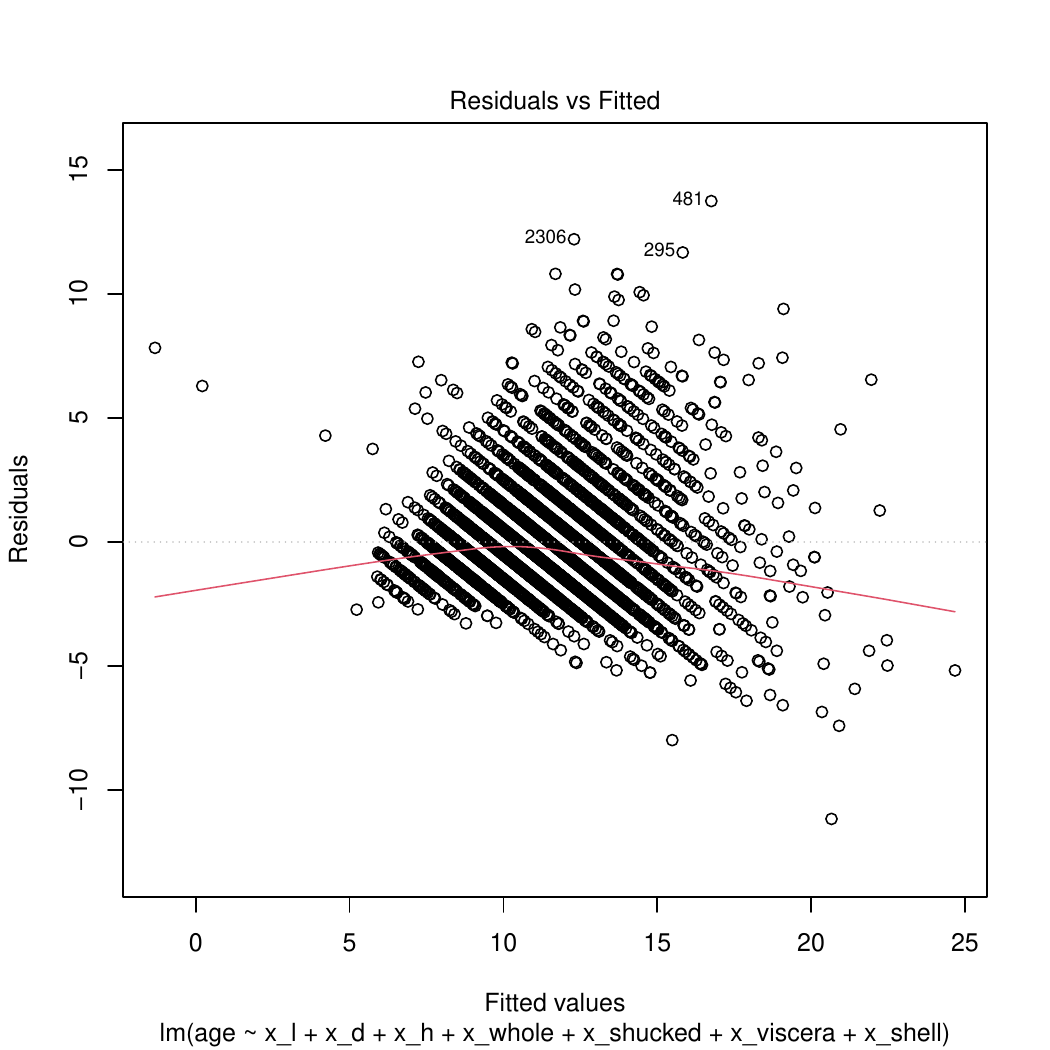
\includegraphics[width=0.49\textwidth]{figures/lm.step-1.png}
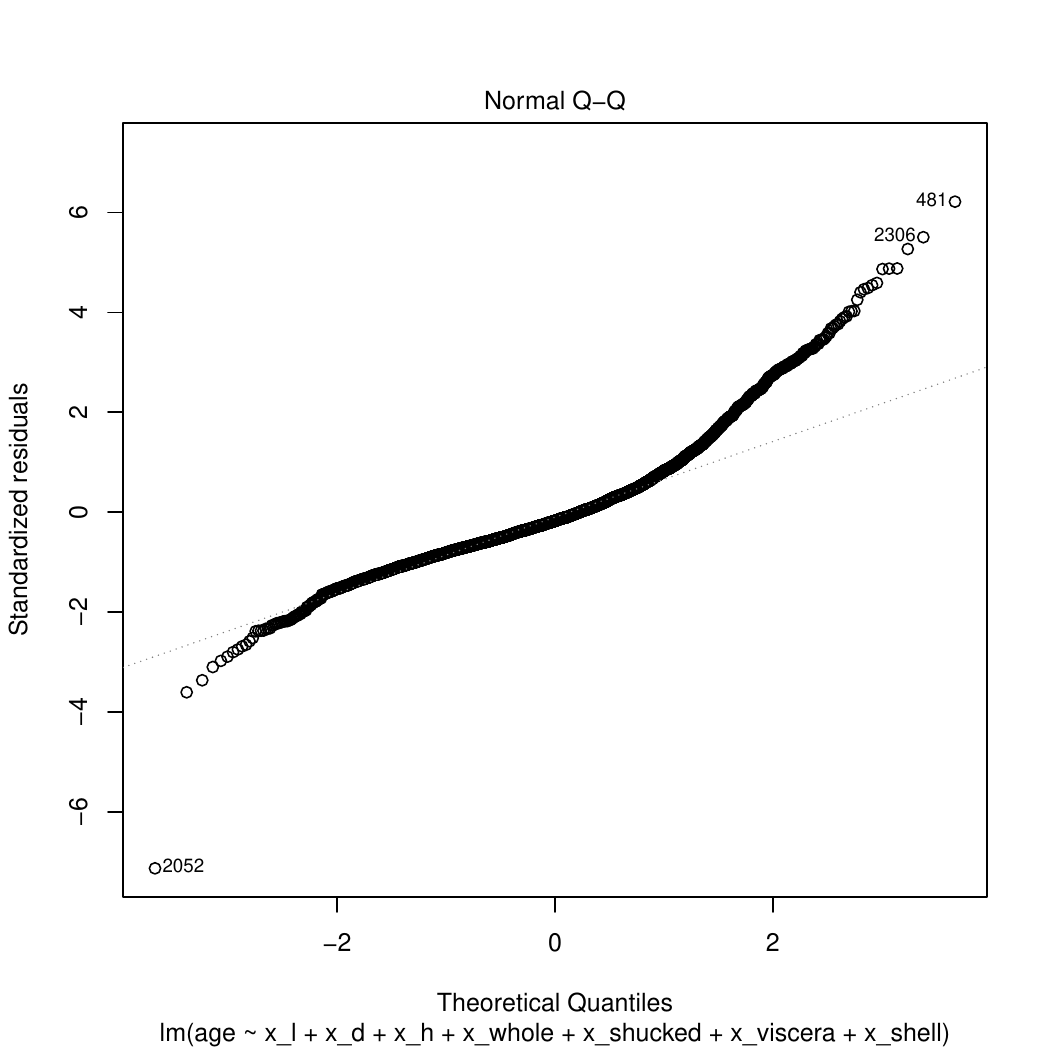
\includegraphics[width=0.49\textwidth]{figures/lm.step-2.png}
\caption{公式 \ref{eq:step} 的残差分布图和 Q-Q 图}
\label{fig:lm_residuals}
\end{figure}

从 Q-Q 图中可以看出,有很大一部分数据都偏离了直线,因此公式的误差很明显。

\section{其他结果}

对于全体鲍鱼的结果不尽人意,但是如果我们试着将鲍鱼简单分类之后会得到一些其他的结果。

\subsection{按照性别分类}

我们将鲍鱼按照性别进行分类,对于不同性别的鲍鱼分别去进行回归分析。

最终发现,性别为 M 的鲍鱼的年龄与其他各项参数的相关性都很弱,大部分都在 $0.5$ 以下。最终得出的回归方程的 $R$ 平方为 $0.4396$。

而性别为 F 的鲍鱼的年龄与其他各项参数的相关性更加弱,大部分都处于 $0.3$ 以下。最终得出的回归方程的 $R$ 平方为 $0.3572$。

而对于性别为 I 的鲍鱼则出现了不一样的情况,鲍鱼的年龄参数和其他各项参数的相关性都比较强,大部分都处于 $0.6$ 以上,但是却没有到达 $0.8$ 的参数。另外最终得出的回归方程的 $R$ 平方为 $0.5875$,比上文中 \ref{eq:step} 的 $R$ 平方 $0.5275$ 要略高一筹,并且平均估计误差也降低到了 $1.617$ 年。

该回归方程为:

\begin{equation} \label{eq:sex_i}
  age = \begin{bmatrix} 4.3214 \\   2.8837 \\   28.5060 \\   8.2473 \\ -14.7666 \\ -11.4193 \\  10.6341 \end{bmatrix} ^{T} \begin{bmatrix} 1 \\ x_d \\ x_h \\ x_{whole} \\ x_{shucked} \\ x_{viscera} \\ x_{shell} \end{bmatrix}
\end{equation}

\subsection{实际情况的应用}

考虑到公式的实际应用场景,我们更加希望通过一些简单测量的数据来估算出鲍鱼的年龄,因此我们将参数限定为前 $4$ 个容易测量的参数(即长度、直径、高度以及整体重量),并进行回归分析,可以得到以下结果:

\begin{equation} \label{eq:real}
  age = \begin{bmatrix} 4.3365 \\ -11.9327 \\ 25.7661 \\ 20.3582 \end{bmatrix} ^{T} \begin{bmatrix} 1 \\ x_l \\ x_d \\ x_h \end{bmatrix}
\end{equation}

这个回归方程的 $R$ 平方仅为 $0.3555$,平均估计误差为 $2.589$ 年。也许方程的估计不够精确,但是它所使用的参数都是非常容易测量的值,因此也许会比方程 \ref{eq:step} 的实际应用面要更广一些。

\section{结论}

文章从一份鲍鱼的数据集中分析得到以下有用的结论可以用于预测鲍鱼的年龄:

\begin{enumerate}
  \item 首先如果当前鲍鱼的性别为 I,则可以使用方程 \ref{eq:sex_i} 来估算鲍鱼的年龄;
  \item 否则可以使用方程 \ref{eq:step} 来比较精确地估算鲍鱼的年龄;
  \item 如果嫌麻烦则可以使用方程 \ref{eq:real} 来粗略地估算鲍鱼的年龄,其准确度也最低。
\end{enumerate}


% 参考文献

\bibliographystyle{plain}

\begin{thebibliography}{99}
\bibitem{a} 第一个参考文献喵
\bibitem{b} 第二个参考文献喵
\end{thebibliography}


% 附录
\appendix
\section{这里是附录喵}

附录里面也一样的喵


\end{document}
